\documentclass[12pt,t]{beamer}
\usetheme{m}

%\usepackage[T1]{fontenc}
%\usepackage[utf8]{inputenc}
\usepackage{microtype}
\usepackage[backend=biber]{biblatex}
\usepackage{graphicx}

\usepackage{nameref}
\makeatletter
\newcommand*{\currentname}{\@currentlabelname}
\makeatother

\beamertemplatenavigationsymbolsempty
\setbeameroption{hide notes}
\setbeamertemplate{note page}[plain]
\setbeamertemplate{caption}{\raggedright\insertcaption\par}


\title{i-score}
\subtitle{Scoring time and interactivity}
\date{Novembre 2015}
\author{Théo de la Hogue\inst{1} \and Pierre Cochard\inst{2} \and Jean-Michaël Celerier\inst{3}}

\institute{\inst{1} GMEA \and \inst{2} LaBRI - SCRIME \and \inst{3} LaBRI - Blue Yeti}

\begin{document}
   
\maketitle

\section{Presentation, Demo, Future}
\begin{frame}{i-score}
    \frametitle{i-score}
    \begin{itemize}
        \item Generalist tree-based data sequencer.
        \item Target : authoring of interaction-heavy content.
        \item Applications : interactive shows, music, museography.
        \item Execution semantics based on formal models.
    \end{itemize}
\end{frame}

\subsection{History}
\begin{frame}
    \frametitle{\currentname}
    \centering
    \begin{figure}
        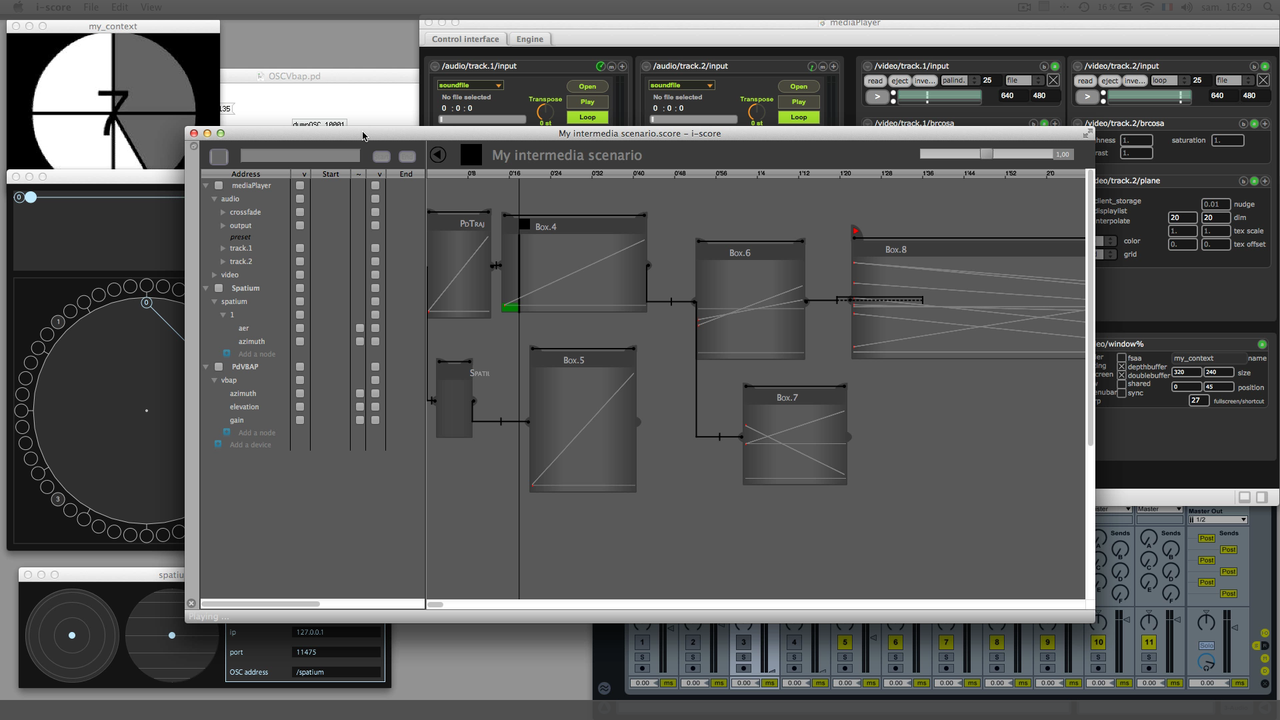
\includegraphics[scale=0.25]{images/02.png}
        \caption{Old i-score}
    \end{figure}
\end{frame}

\begin{frame}
    \frametitle{\currentname}
    \centering
    \begin{figure}
        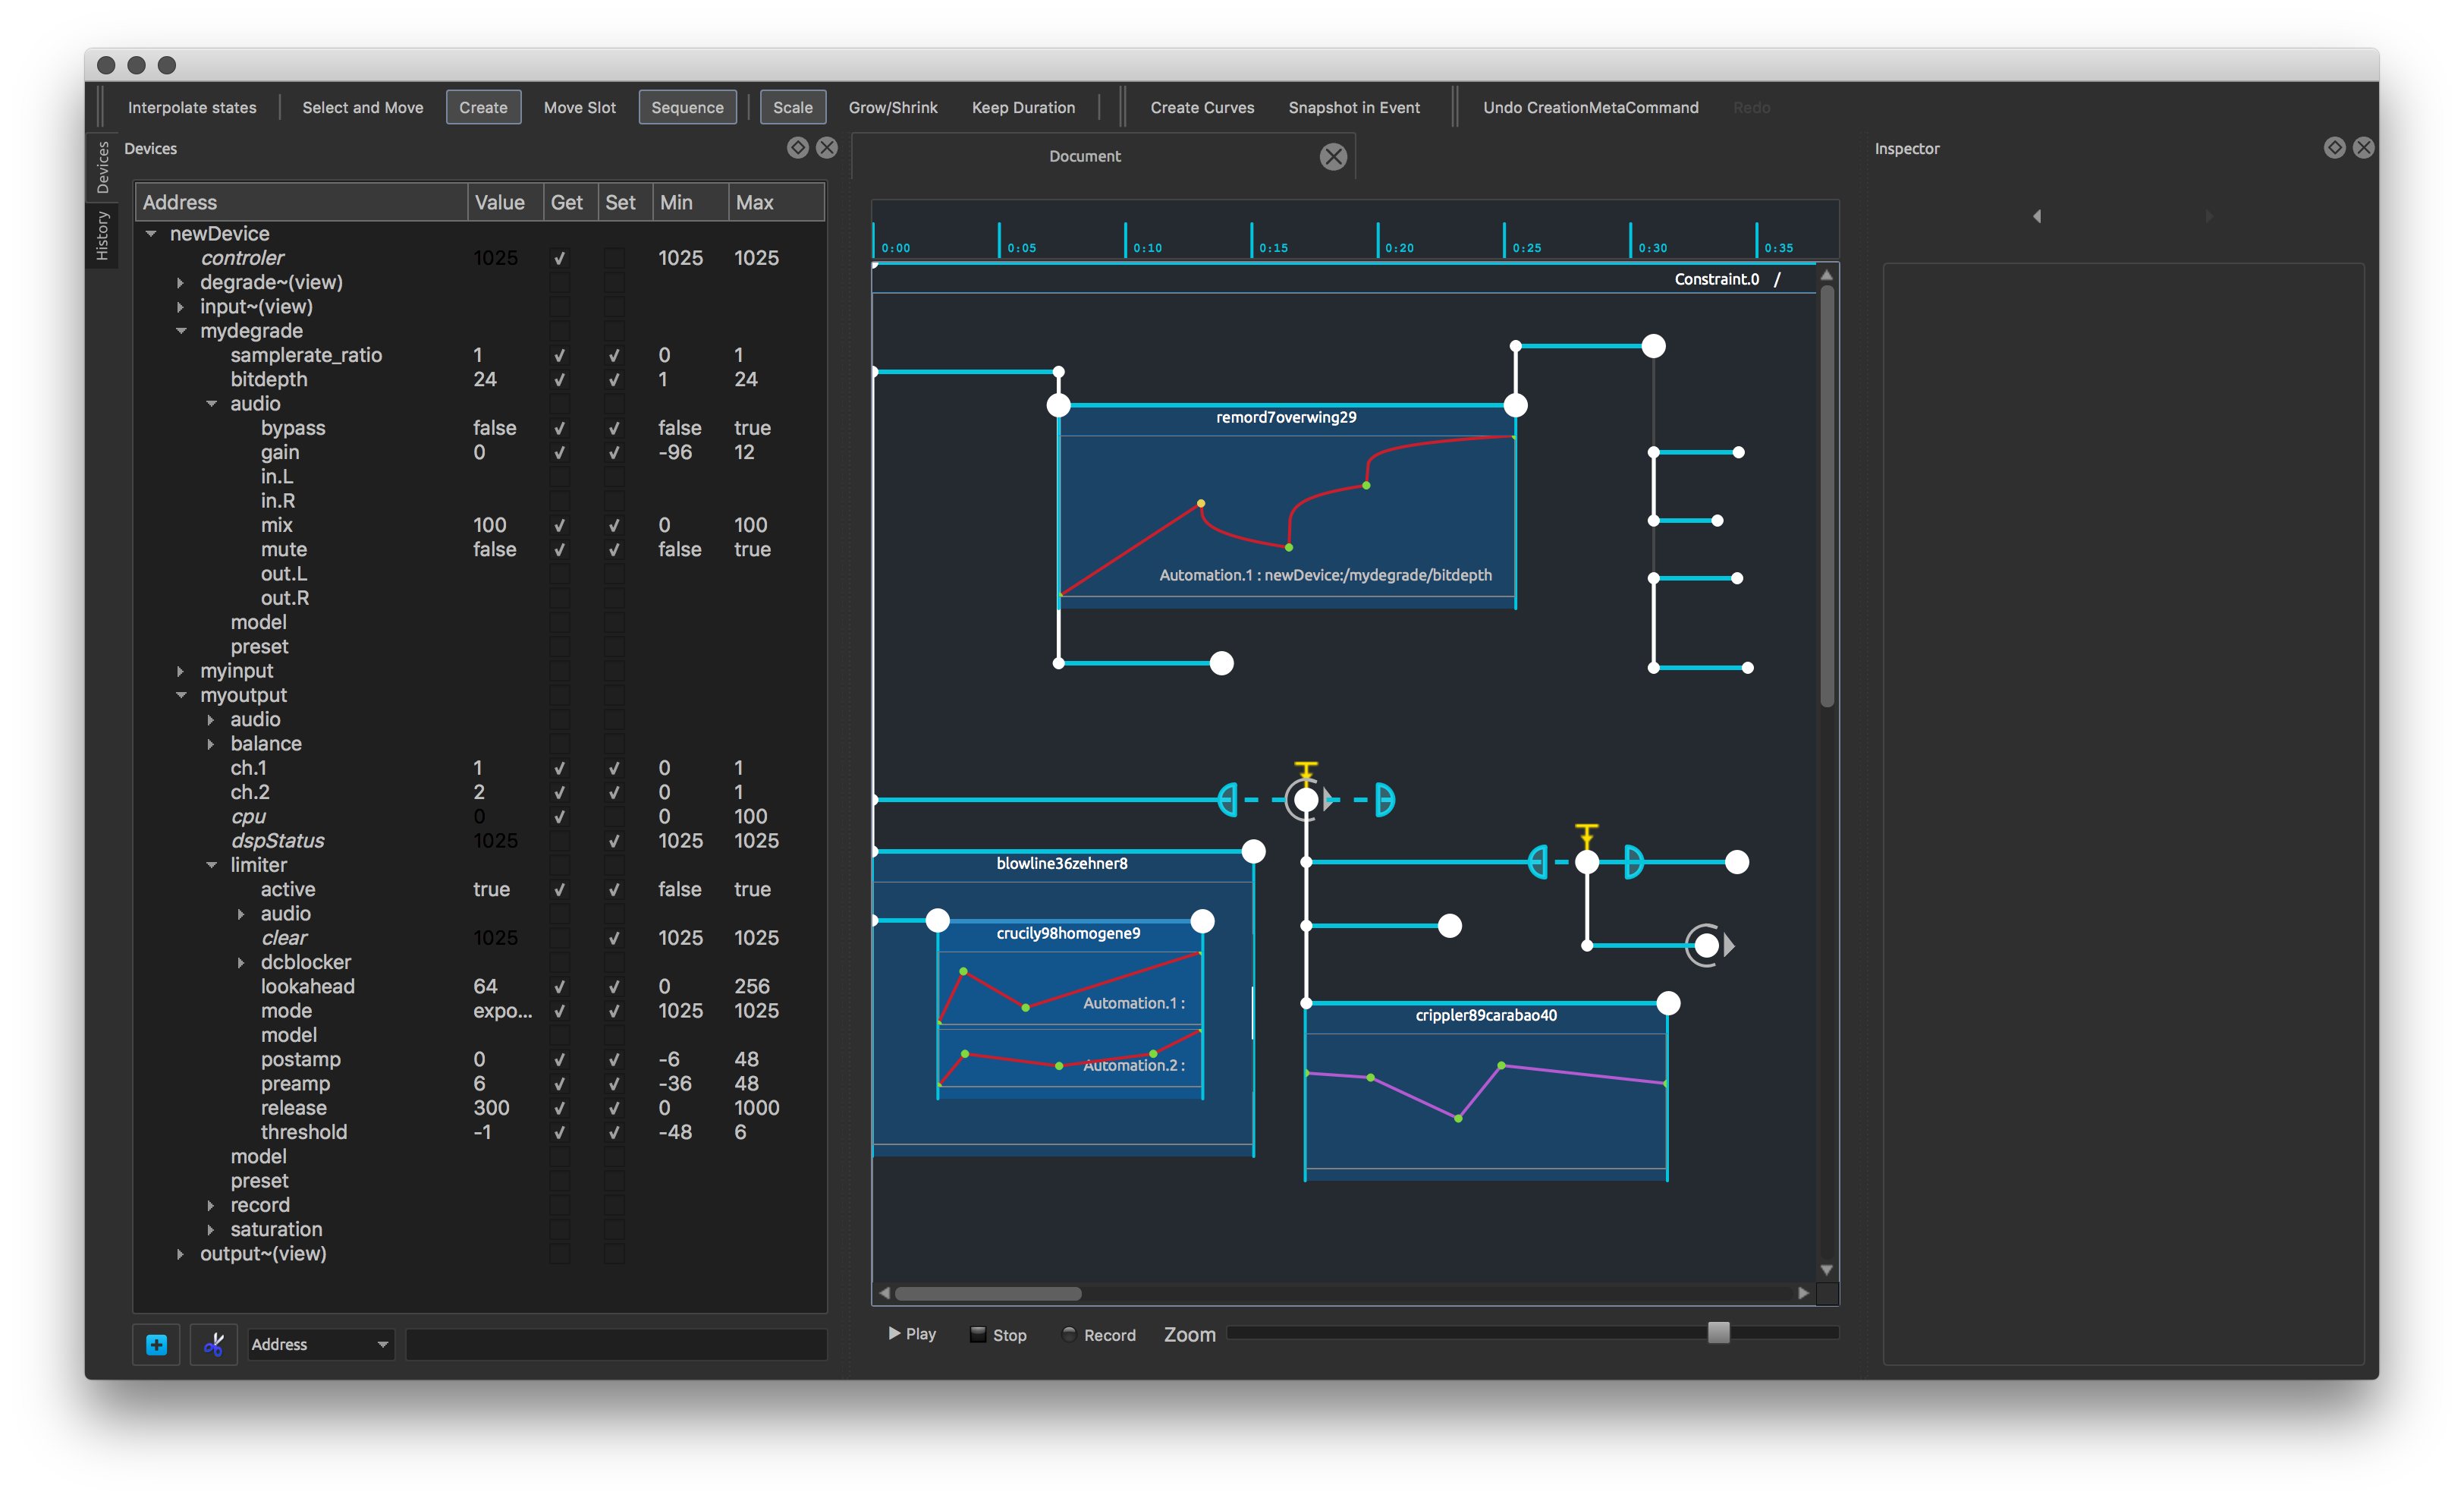
\includegraphics[scale=0.20]{images/General.png}
        \caption{New i-score}
    \end{figure}
\end{frame}

\subsection{Graphical chart}
\begin{frame}
    \frametitle{\currentname}
    \centering
    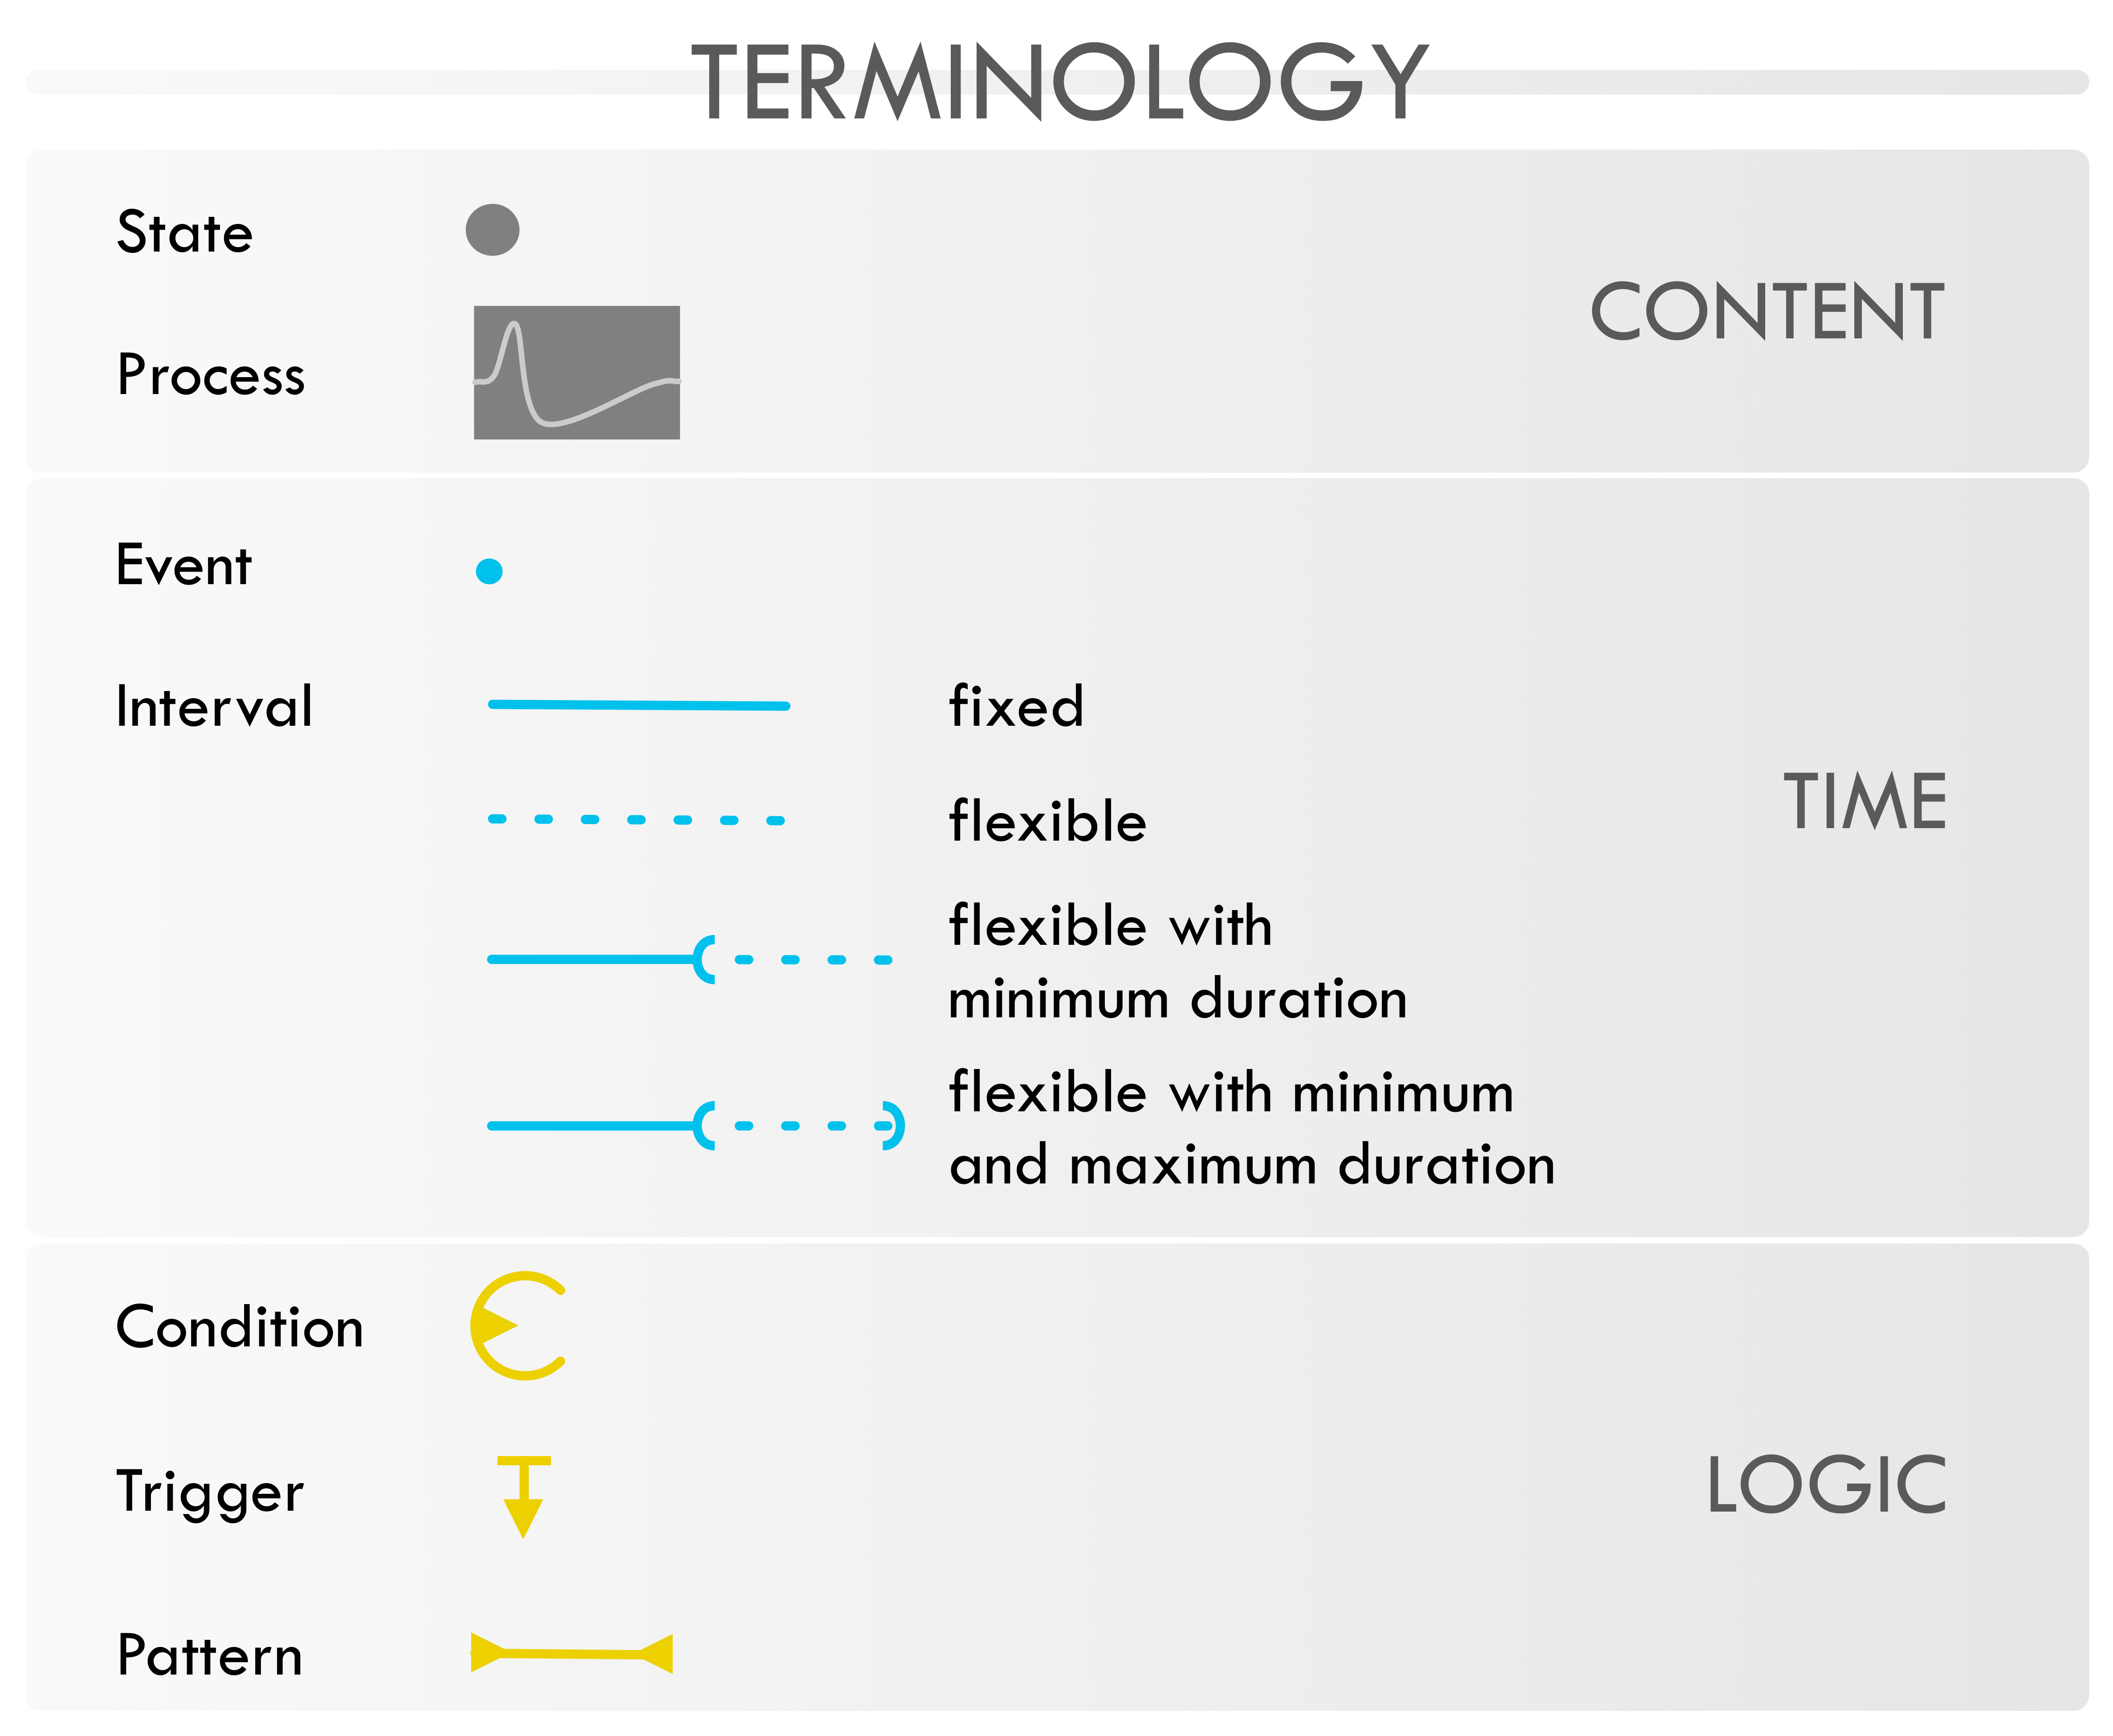
\includegraphics[scale=0.057]{images/terminology.jpg}
\end{frame}
\begin{frame}
    \frametitle{\currentname}
    \centering
    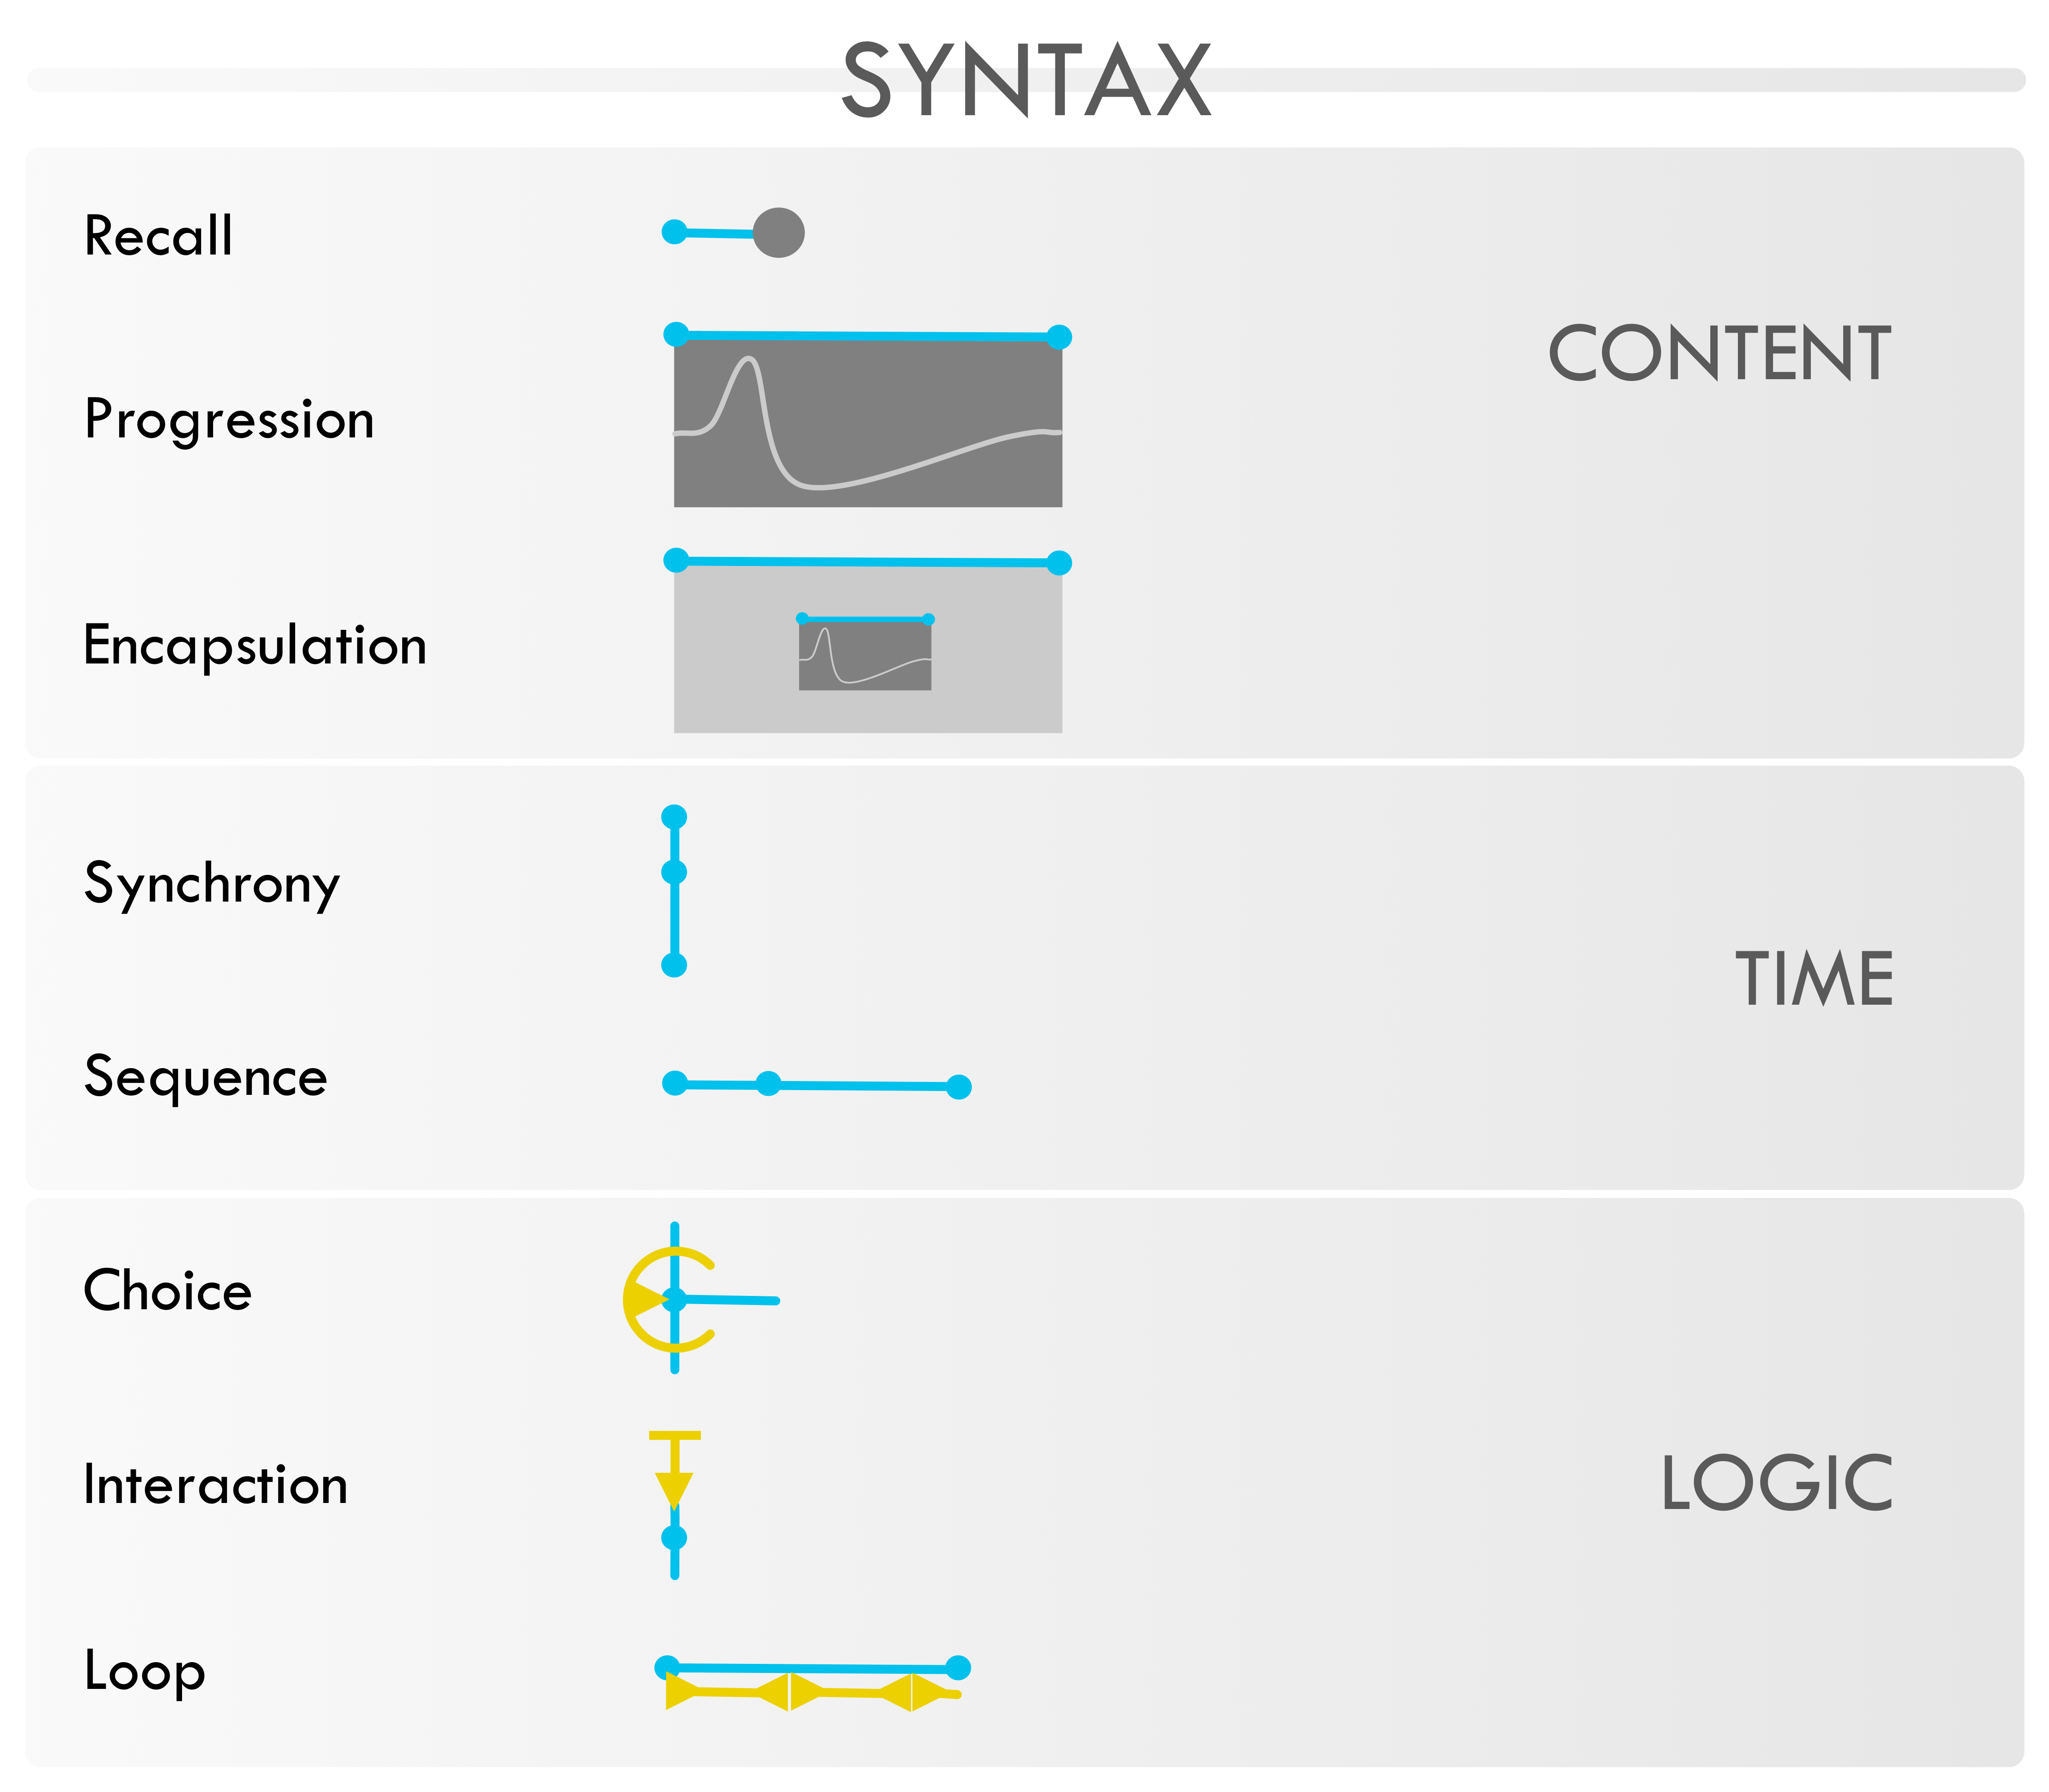
\includegraphics[scale=0.055]{images/syntax.jpg}
\end{frame}
\begin{frame}
    \frametitle{\currentname}
    \centering
    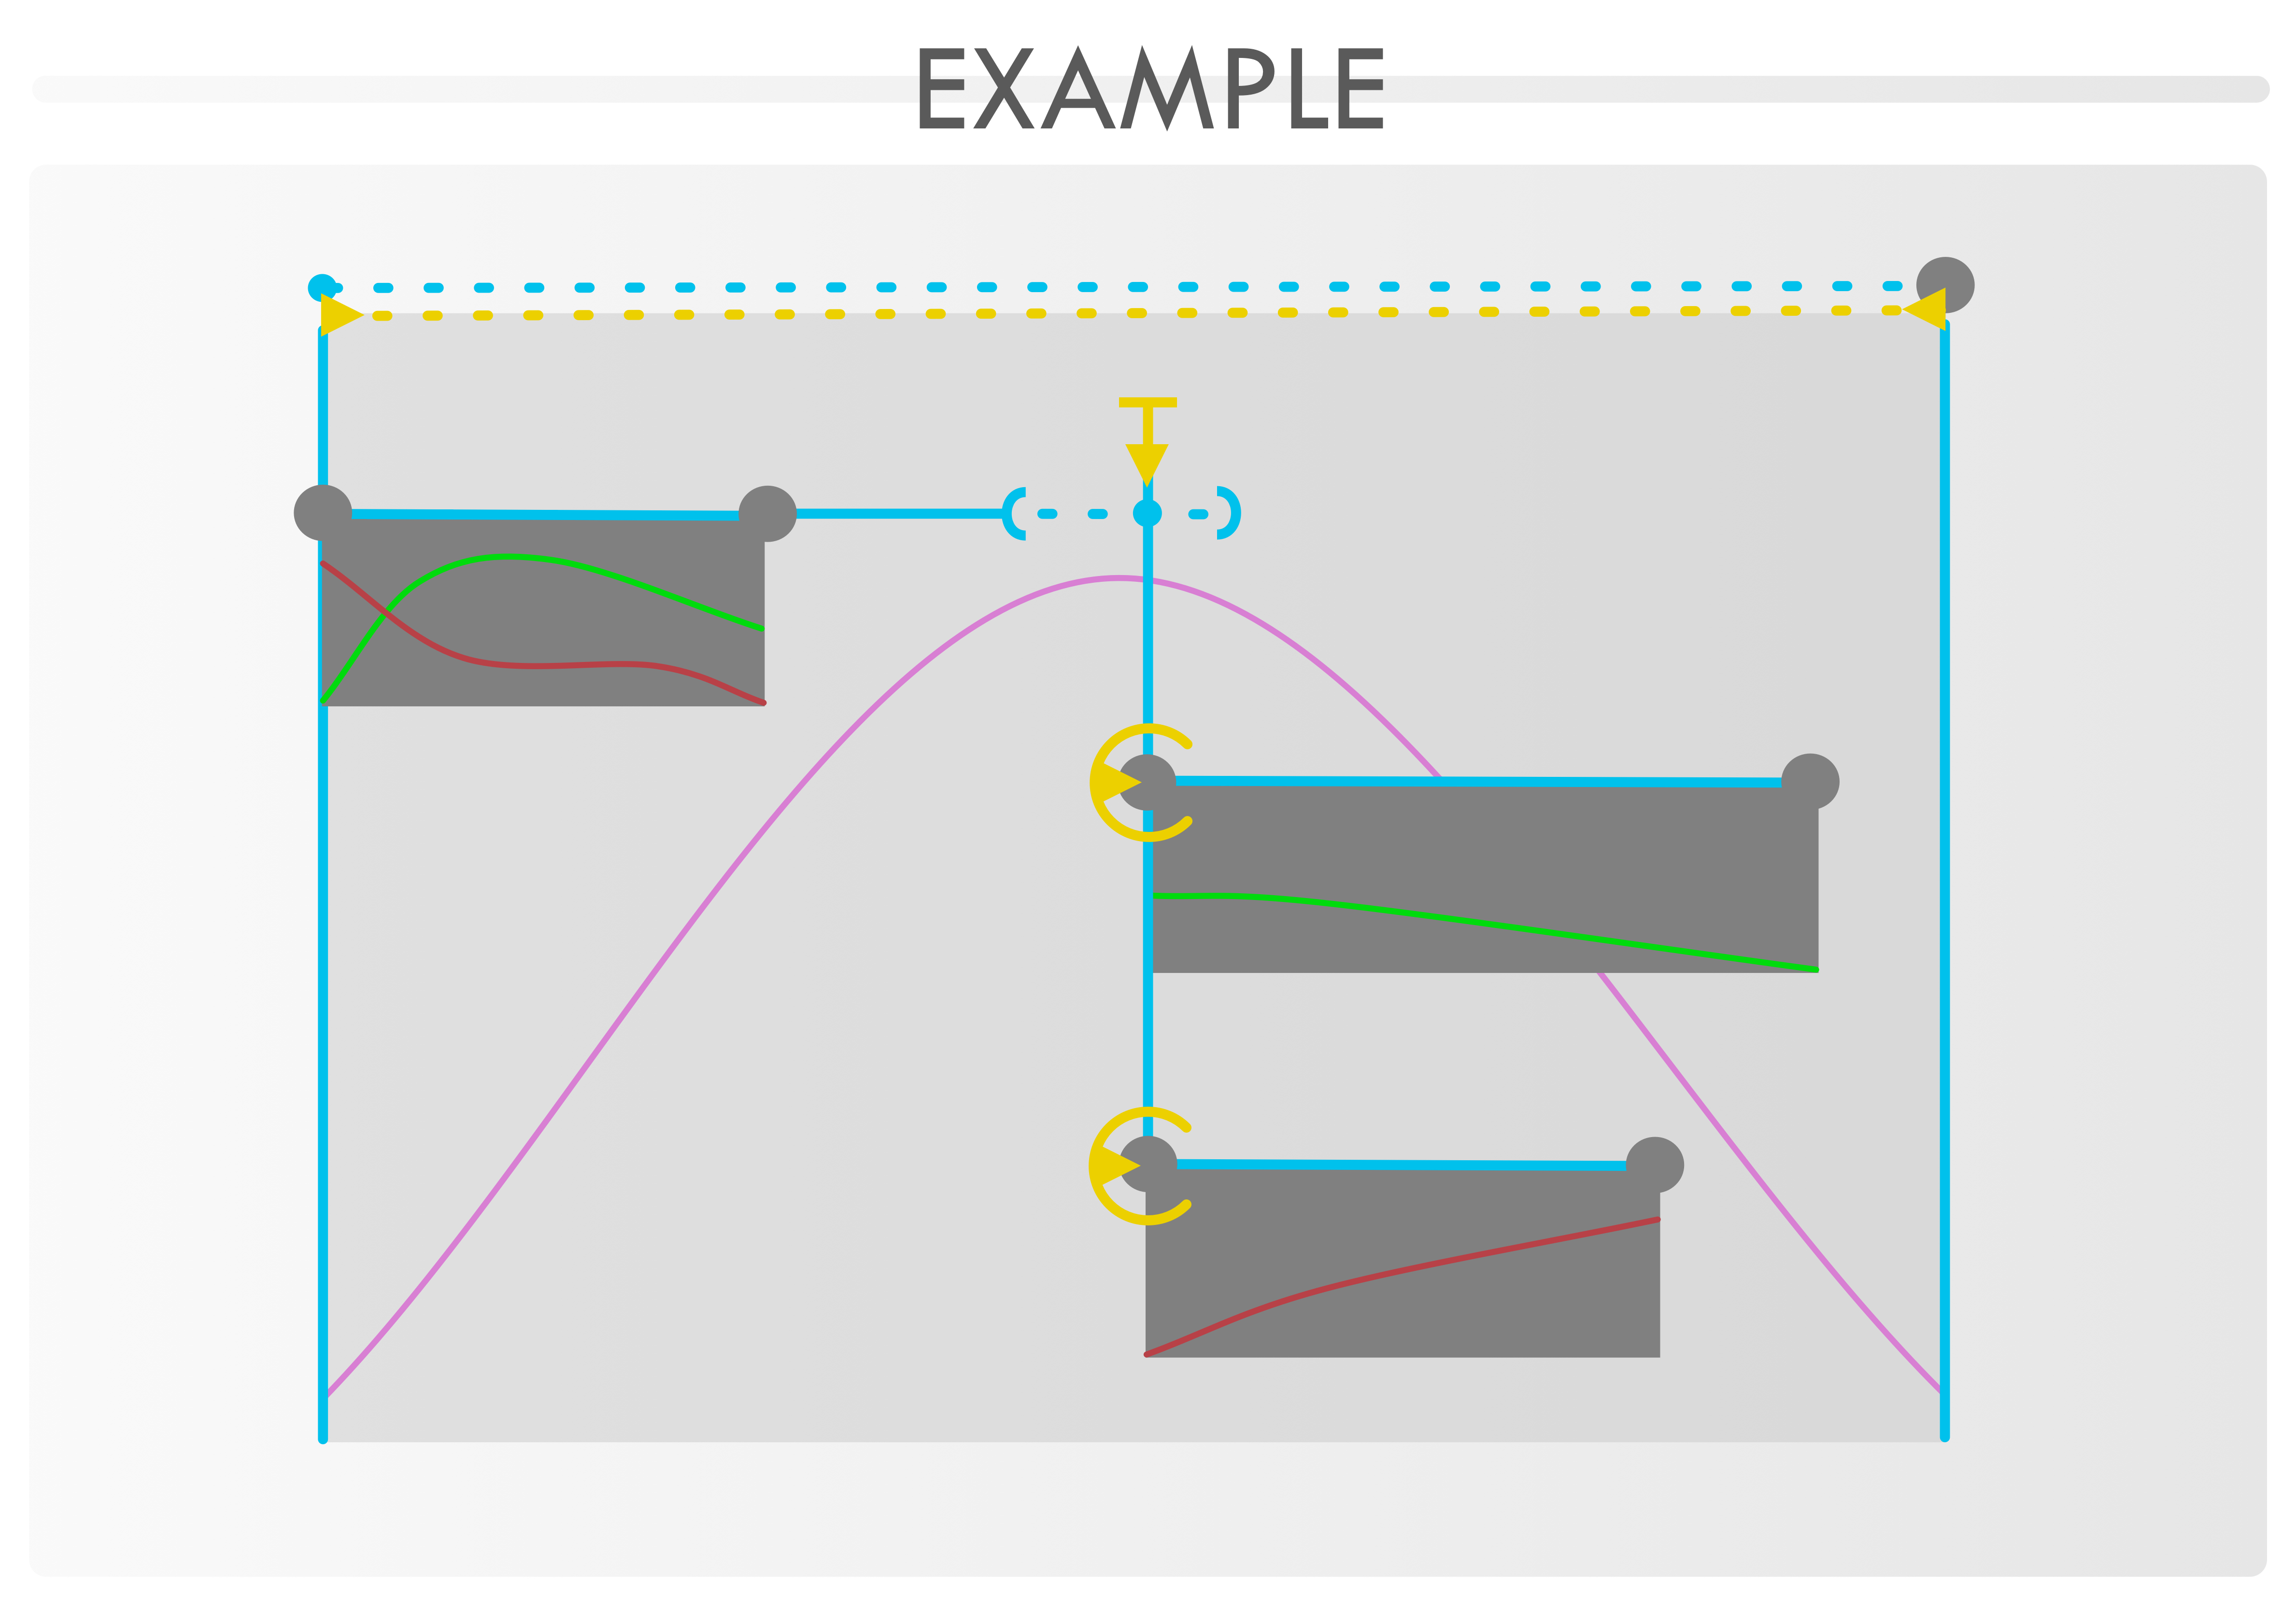
\includegraphics[scale=0.065]{images/example.jpg}
\end{frame}

\subsection{Features}
\begin{frame}
    \frametitle{\currentname}
    \begin{itemize}
        \item Hierarchy, automations, mappings, custom \textbf{Javascript} execution.
        \item Protocols : \textbf{OSC}, \textbf{Minuit}. \textbf{MIDI}, \textbf{OSCQuery} in progress.
        \item Multiple plug-in interfaces for extensibility.
        \item Collaborative editing.
        \item Works on \textbf{OS X}, \textbf{Windows}, \textbf{Linux} (desktop and embedded), \textbf{Android}.
        \item Integration to Max/MSP and command-line player (in progress).
        \item Web visualisation of execution (in progress).
    \end{itemize}
\end{frame}


\subsection{Minuit integrations}
\begin{frame}
    \frametitle{\currentname}
    \centering
    \begin{figure}
        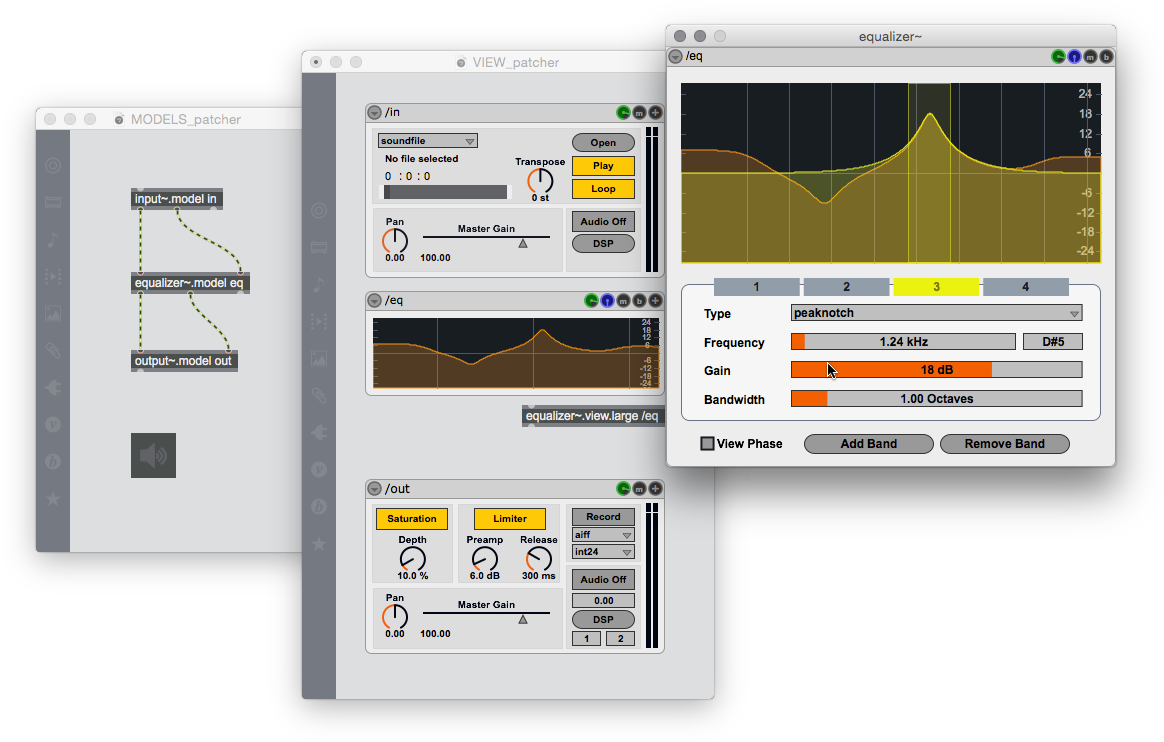
\includegraphics[scale=0.2]{images/jamoma.png}
        \caption{Max/MSP with Jamoma}
    \end{figure}
\end{frame}

\begin{frame}
    \frametitle{\currentname}
    \centering
    \begin{figure}
        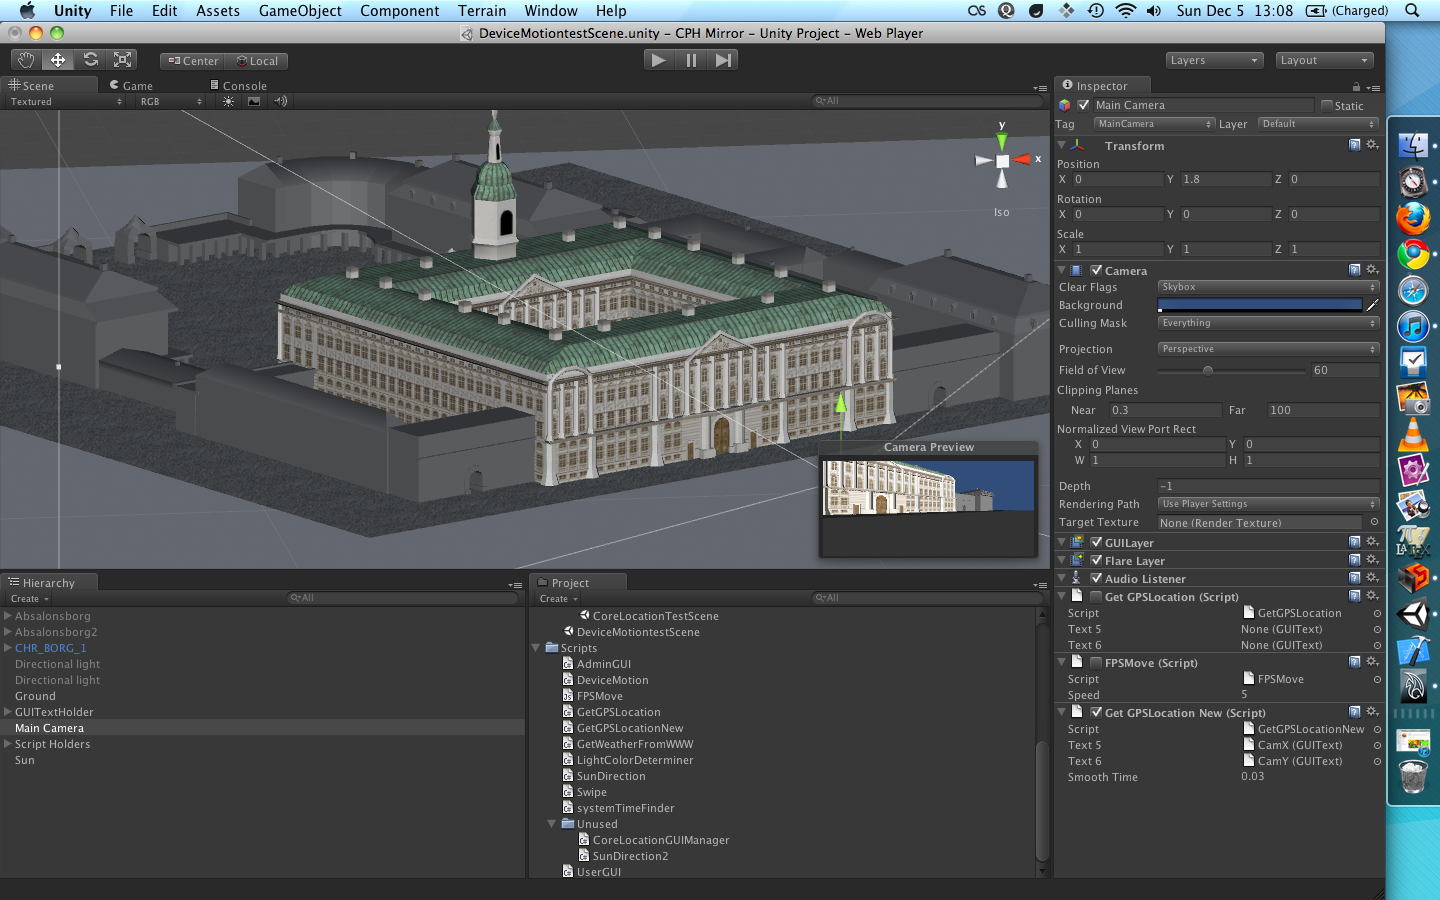
\includegraphics[scale=0.2]{images/unity.png}
        \caption{Unity}
    \end{figure}
\end{frame}

\begin{frame}
    \frametitle{\currentname}
    \centering
    \begin{figure}
        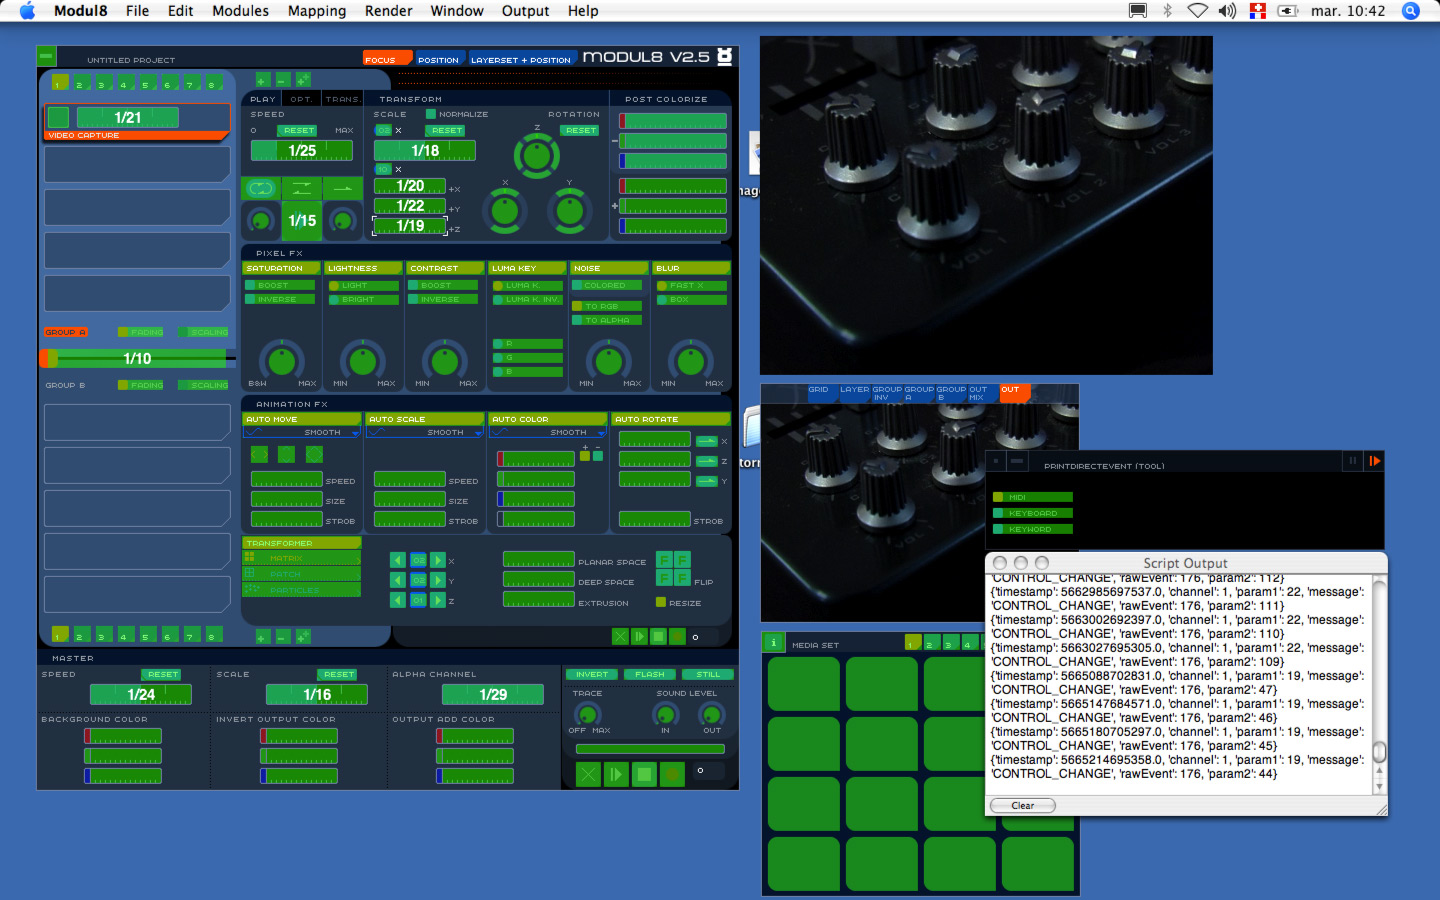
\includegraphics[scale=0.2]{images/modul8.jpg}
        \caption{Modul8}
    \end{figure}
\end{frame}


\subsection{Demo}


\subsection{Perspectives}
\begin{frame}
    \frametitle{\currentname}
    \begin{itemize}
        \item \textbf{Spatial data authoring} :
        
        \begin{itemize}
            \item For audio trajectories, video games, interactive kiosks.
            \item Generalized mapping between any parameters. 
            \item The created structures can influence each other and properties can be 
            extracted (such as collisions, etc.).
            \item Collaborate with IanniX ?
        \end{itemize}
        
        \item \textbf{Sound} : 
        \begin{itemize}
            \item Integrating i-score with FaUST / libaudiostream (in progress).
            \item It would allow "Audio" processes that would behave like traditional DAW tracks.
        \end{itemize}
    \end{itemize}
\end{frame}

\begin{frame}
    \frametitle{Links}
    \begin{itemize}
        \item \textbf{Stable} (old) :~\\ \url{www.i-score.org}.
        \item \textbf{Alpha} (this) :~\\ \url{github.com/OSSIA/i-score/releases}. 
    \end{itemize}
    
    We welcome contributions (GPL-v3).
    
    \centering
    \vspace{2cm}
    \Large{Thanks !}
\end{frame}


\end{document}
